\subsubsection{Planificación inicial} \label{sec:5-Planificacion-inicial}
\hypertarget{sec:5-Planificacion-inicial}{}
A partir de las tareas definidas en la sección \coloredUnderline{\hyperlink{sec:5-WBS}{\ref*{sec:5-WBS} \nameref*{sec:5-WBS}}} se ha realizado una planificación inicial del proyecto, en la que se han establecido las fechas de inicio y fin de cada tarea, así como su duración y las dependencias entre ellas. 
La planificación inicial se ha realizado en la herramienta \coloredUnderline{\href{hhttps://www.microsoft.com/es-es/microsoft-365/p/project-profesional-2019/cfq7ttc0k7cj}{Microsoft Project}}.
Al igual que en la sección anterior, se ha dividido la planificación en las fases en las que se divide el proyecto para mejorar la legibilidad mostrando primero una visión general y después entrando en detalle en cada una de las fases.
Se incluye una tabla con las siguientes columnas:
\begin{itemize}
    \item \textbf{EDT:} Estructura de Desglose del Trabajo, también conocida como WBS. Detalla el identificador de la tarea.
    \item \textbf{Nombre tarea:} Nombre de la tarea.
    \item \textbf{Duración:} Duración de la tarea en horas.
    \item \textbf{Fecha inicio:} Fecha de inicio de la tarea.
    \item \textbf{Fecha fin:} Fecha de fin de la tarea.
\end{itemize}

\subsubsubsection{Planificación inicial. Visión general}
En la \coloredUnderline{\hyperlink{table:5_PI-Vision-General}{\ref*{table:5_PI-Vision-General}: \nameref*{table:5_PI-Vision-General}}} se muestra la planificación inicial del proyecto de alto nivel, es decir, las tareas generales o fases que se deben realizar para cumplir con los objetivos del proyecto.
El total de días estimados para la realización del proyecto es de 71,13 días (462 horas), desde el 01/04/2024 hasta el 18/06/2024.


\begin{table}[H]
    \centering
    \caption{Planificación inicial. Visión general}
    \label{table:5_PI-Vision-General}
    \hypertarget{table:5_PI-Vision-General}{}
    \begin{tabular}{
       >{\columncolor{lightgreen!20}\raggedright\arraybackslash}p{1.5cm}
       >{\raggedright\arraybackslash}p{4.5cm}
       >{\raggedright\arraybackslash}p{2cm}
       >{\raggedright\arraybackslash}p{3cm}
       >{\raggedright\arraybackslash}p{3cm} }
    \rowcolor{darkgreen!50}
    \toprule
    \textbf{EDT} & \textbf{Nombre tarea} & \textbf{Duración} & \textbf{Fecha inicio} & \textbf{Fecha fin} \\
    \midrule
    1 & Proyecto BidMon Universe & 462 horas & 01/04/2024 & 18/06/2024 \\
    \midrule
    1.1 & Análisis del proyecto & 12 horas & 01/04/2024 & 12/04/2024 \\
    \midrule
    1.2 & Seguimiento del proyecto & 30,5 horas & 01/04/2024 & 18/06/2024 \\
    \midrule
    1.3 & Diseño del sistema & 76 horas & 03/04/2024 & 15/05/2024 \\
    \midrule
    1.4 & Implementación del sistema &  156,5 horas & 03/04/2024 & 22/05/2024 \\
    \midrule
    1.5 & Fase de pruebas & 9 horas & 28/05/2024 & 01/06/2024 \\
    \midrule
    1.6 & Despliegue del sistema & 8 horas & 12/06/2024 & 13/06/2024 \\
    \midrule
    1.7 & Documentación del proyecto & 170 horas & 02/04/2024 & 18/06/2024 \\
    \bottomrule
    \end{tabular}
\end{table}

A continuación, se muestra la línea temporal de las tareas del proyecto en la \coloredUnderline{\hyperlink{fig:5_PI-Linea-Temporal}{Figura \ref*{fig:5_PI-Linea-Temporal}: \nameref*{fig:5_PI-Linea-Temporal}}}.
Mediante esta planificación se pretende priorizar las tareas de análisis y diseño del sistema, para posteriormente realizar la implementación y las pruebas del sistema, y finalmente desplegar el sistema. 
La fase de documentación del proyecto se realizará de forma paralela a las demás tareas al igual que el seguimiento del proyecto.
\begin{figure}[H]
    \hypertarget{fig:5_PI-Linea-Temporal}{}
    \centering
    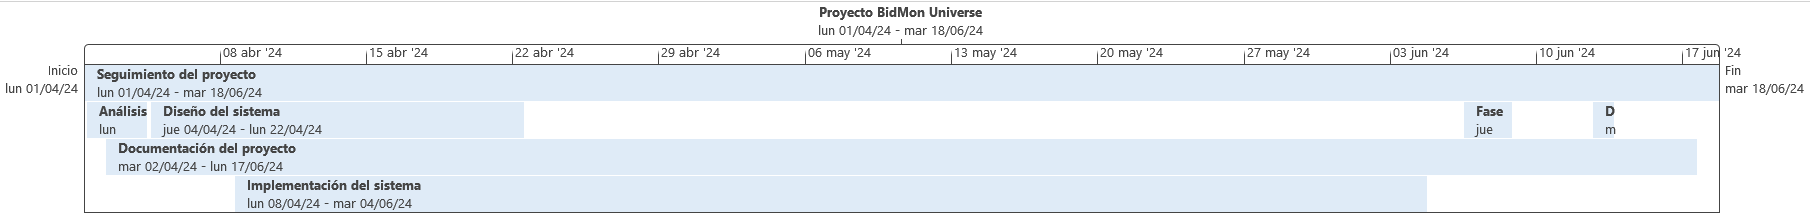
\includegraphics[width=1\linewidth]{figures/5_PI-Linea-Temporal.png}
    \caption{Planificación inicial. Línea temporal}
    \label{fig:5_PI-Linea-Temporal}
\end{figure}



\subsubsubsection{Planificación inicial. Análisis del proyecto}
En la \coloredUnderline{\hyperlink{table:5_PI-Analisis}{\ref*{table:5_PI-Analisis}: \nameref*{table:5_PI-Analisis}}}, se detallan la planificación de las tareas que se deben realizar en la fase de análisis del sistema.
El total de días estimados para la realización de esta fase es de 12 horas, desde el 01/04/2024 hasta el 12/04/2024.
\begin{table}[H]
    \centering
    \caption{Planificación inicial. Análisis del proyecto}
    \label{table:5_PI-Analisis}
    \hypertarget{table:5_PI-Analisis}{}
    \begin{tabular}{
       >{\columncolor{lightgreen!20}\raggedright\arraybackslash}p{1.5cm}
       >{\raggedright\arraybackslash}p{4.5cm}
       >{\raggedright\arraybackslash}p{2cm}
       >{\raggedright\arraybackslash}p{3cm}
       >{\raggedright\arraybackslash}p{3cm} }
    \rowcolor{darkgreen!50}
    \toprule
    \textbf{EDT} & \textbf{Nombre tarea} & \textbf{Duración} & \textbf{Fecha inicio} & \textbf{Fecha fin} \\
    \midrule
    1.1 & Análisis del proyecto & 12 horas & 01/04/2024 & 12/04/2024 \\
    \midrule
    1.1.1 & Análisis del sistema & 5 horas & 01/04/2024 & 02/04/2024 \\
    \midrule
    1.1.2 & Análisis de la arquitectura & 3 horas & 11/04/2024 & 11/04/2024 \\
    \midrule
    1.1.3 & Análisis de la infraestructura & 4 horas & 12/04/2024 & 12/04/2024 \\
    \midrule
    1.1.4 & Determinación del análisis & 2 horas & 12/04/2024 & 12/04/2024 \\
    \bottomrule
    \end{tabular}
\end{table}

\subsubsubsection{Planificación inicial. Seguimiento del proyecto}
En la \coloredUnderline{\hyperlink{table:5_PI-Seguimiento}{\ref*{table:5_PI-Seguimiento}: \nameref*{table:5_PI-Seguimiento}}}, se detalla la planificación de las tareas que se deben realizar en la fase de seguimiento del proyecto.
El total de días estimados para la realización de esta fase es de 30,5 horas, desde el 01/04/2024 hasta el 18/06/2024, abarca todo el proyecto debido a que se realiza una reunión inicial, reuniones periódicas y una reunión final para la revisión del proyecto.
\begin{table}[H]
    \centering
    \caption{Planificación inicial. Seguimiento del proyecto}
    \label{table:5_PI-Seguimiento}
    \hypertarget{table:5_PI-Seguimiento}{}
    \begin{tabular}{
       >{\columncolor{lightgreen!20}\raggedright\arraybackslash}p{1.5cm}
       >{\raggedright\arraybackslash}p{4.5cm}
       >{\raggedright\arraybackslash}p{2cm}
       >{\raggedright\arraybackslash}p{3cm}
       >{\raggedright\arraybackslash}p{3cm} }
    \rowcolor{darkgreen!50}
    \toprule
    \textbf{EDT} & \textbf{Nombre tarea} & \textbf{Duración} & \textbf{Fecha inicio} & \textbf{Fecha fin} \\
    \midrule
    1.2 & Seguimiento del proyecto & 30,5 horas & 01/04/2024 & 12/04/2024 \\
    \midrule
    1.2.1 & Reunión de arranque & 2 horas & 01/04/2024 & 01/04/2024 \\
    \midrule
    1.2.2 & Reuniones periódicas & 20,5 horas & 27/04/2024 & 30/04/2024 \\
    \midrule
    1.2.3 & Reunión de revisión & 4 horas & 15/06/2024 & 15/06/2024 \\
    \midrule
    1.2.4 & Reunión final & 4 horas & 17/04/2024 & 18/04/2024 \\
    \bottomrule
    \end{tabular}
\end{table}

\subsubsubsection{Planificación inicial. Diseño del sistema}
En la \coloredUnderline{\hyperlink{table:5_PI-Diseno}{\ref*{table:5_PI-Diseno}: \nameref*{table:5_PI-Diseno}}}, se detalla la planificación de las tareas que se deben realizar en la fase de diseño del sistema.
El total de días estimados para la realización de esta fase es de 76 horas, desde el 03/04/2024 hasta el 15/05/2024.
\begin{table}[H]
    \centering
    \caption{Planificación inicial. Diseño del sistema}
    \label{table:5_PI-Diseno}
    \hypertarget{table:5_PI-Diseno}{}
    \begin{tabular}{
       >{\columncolor{lightgreen!20}\raggedright\arraybackslash}p{1.5cm}
       >{\raggedright\arraybackslash}p{4.5cm}
       >{\raggedright\arraybackslash}p{2cm}
       >{\raggedright\arraybackslash}p{3cm}
       >{\raggedright\arraybackslash}p{3cm} }
    \rowcolor{darkgreen!50}
    \toprule
    \textbf{EDT} & \textbf{Nombre tarea} & \textbf{Duración} & \textbf{Fecha inicio} & \textbf{Fecha fin} \\
    \midrule
    1.3 & Diseño del sistema & 76 horas & 03/04/2024 & 15/05/2024 \\
    \midrule
    1.3.1 & Diseño del \textit{backend} & 22 horas & 03/04/2024 & 16/04/2024 \\
    \midrule


    \bottomrule
    \end{tabular}
\end{table}